% !TeX spellcheck = en_US
\documentclass[parskip=full]{report}

\usepackage{amsmath}
\usepackage{listings}
%\usepackage{beramono}
\usepackage{float}
\usepackage[utf8]{inputenc}
\usepackage[T1]{fontenc}
\usepackage{xcolor}
\usepackage[a4paper, margin={3cm}]{geometry}
\usepackage{hyperref}
\usepackage{graphicx}
\usepackage{subcaption}
\usepackage{float}


%\usepackage{hyphenat}
%\usepackage[english]{babel}
% Carattere monospaziato di default
%\renewcommand{\ttdefault}{pcr}

\lstset{
	tabsize=2,
	basicstyle=\ttfamily\small,
	numbers=left,
	rulecolor=\color{black!30},
	escapeinside={\%TEX}{\^^M},
	inputencoding=utf8,
	extendedchars=true,
	literate={á}{{\'a}}1 {à}{{\`a}}1 {é}{{\'e}}1 {è}{{\`e}}1,
}


% Title Page
\title{
	
\includegraphics[width=0.333\textwidth]{assets/unipi1.png} \\
	London Safe Travel
}

\author{
	Dario Pagani, 585281 \\
	Federico Frati, 596237\\
	Ricky Marinsalda, 585094
}


\begin{document}
\maketitle
\tableofcontents


\part{Introduction}

\paragraph{}
Every day millions of people find themselves in the troublesome task of 
computing a route to their desired destination. We'll provide directions for 
their journey with state of the art routing algorithms in a safe way. The 
service will provide the following transportation modes when querying a route: 
car, foot and bicycle. We’ll also provide a compact and easy way to view 
timetables and public transport’s routes.

\paragraph{Problem}
Navigating a city like London is a complicated matter even during normal times, 
let alone during rush hour. Due to the convoluted nature of London’s road 
network accidents and disruptions are common occurrences that afflict all road 
users during their journeys [?]. People who use public transportation to travel 
around the city could be interested in knowing which are the most congested 
lines in advance in order to avoid delays and other kinds of interference.

\paragraph{Objective}
We’ll provide analytic functionalities to find hotspots in the road network 
graph, that is to collect information about all users’ journeys and visualize 
the most congested routes/graph’s regions. Other information about public 
transportation’s issues will help users to locate and avoid the most critical 
parts of the transportation network.

% !TeX root = ../report.tex

\part{Feasibility}
\chapter{Data sources}

We’re combining data from three sources and two organizations:

\begin{itemize}
	\item Transport for London TIMS
	\item Transport for London public disruptions API
	\item OpenStreetMap
\end{itemize}

\paragraph{Introduction}
At the very beginning, we made a feasibility study of the project idea, in 
order to identify both the pros and the critical aspects of the application, 
considering the time and technical constraints at the time and thinking how to 
possibly improve our work in future.

\section{Transport for London}

\paragraph{Scraping}
Transport for London provides data at regular intervals – every five 
minutes –  and in a standardized format; this kind of data, especially when 
scrapped during an adequate period of time can provide a good amount of 
information to be analyzed by our application. Those analyses become of 
particular interest when we consider that Transport for London provides 
data with a great amount of detail, including things such as minor collisions 
and broken traffic lights. In our particular case we collected data for circa a 
month using \textit{Transport for London}’s JSON API with a simple shell script 
that was being executed 
automatically by a \textit{SystemD} timer every ten minutes.

\paragraph{Format}
An example 

\paragraph{Schema}
The main challenge was to find a “schema” for the document database to store in 
an unified way, that is to share the same MongoDB collection, between road 
disruptions and public transportation disruptions; as it could be useful for 
certain operations to have an unified view of such data.

\section{OpenStreetMap}

\paragraph{Scraping}
Since the map’s data would be used only for routing purposes, we don’t need all 
the information provided by OpenStreetMap; so, to reduce the dimension of the 
data and maintain only the useful information, we decided to do some pruning of 
the network graph, in particular we removed useless nodes such as buildings, 
waterways, trees, parks and so on.

\paragraph{Schema}
The main challenge was to find a good representation of OpenStreetMap’s data 
for our chosen graph database (Neo4j) because it has to represents facts like 
one ways streets, access restrictions and the elements’ geographical positions; 
we iterate over several possible schemas for the graph database and over many 
different ways to import the raw data into it.

\begin{figure}[H]
	%\lstinputlisting[lastline=5]{../../src/libCommon/examples/nodes.csv}
	\caption{Example of intersections}
\end{figure}


% !TeX root = ../report.tex

\part{Design}

\chapter{Main Actors}
The application has three main actors:
\begin{itemize}
	\item Client
	\item TIMS
	\item Statician
\end{itemize}

\paragraph{Client}
this user is able to view map and run searches on it and he’s also able to ask 
for directions between two points on the map.

\paragraph{TIMS}
this user is able to perform CRUD operations on the disruptions.

\paragraph{Statician}
this user is able to perform analytics on the data generated by TIMS.

\chapter{Functional requirements}
The application will allow its users to perform the following tasks:

\section{Client}

\begin{itemize}
	\item \textbf{View the map}
	\item \textbf{Move the map in a direction}, with the typical drag 'n drop
	\item \textbf{Increase or decrease the map magnifying}, with either buttons 
	or the mouse's wheel
	\item \textbf{Search for a specific place}, the following method are 
	supported:
	\begin{itemize}
		\item With an address
		\item With a POI's name
		\item With WGS84 geographical coordinates
	\end{itemize}
	\item \textbf{Ask for directions} between two intersections on the map
	\begin{itemize}
		\item Via car
		\item Via bicycle
		\item On foot
	\end{itemize}
\end{itemize}
\section{TIMS}
	\begin{itemize}
	\item \textbf{Create/Update a disruption}
	\item \textbf{Close a disruption}
	
	\end{itemize}
\section{Statician}
\begin{itemize}
	\item \textbf{Access the analytics tools}
	\item \textbf{Display the disruptions' heatmap}
\end{itemize}
\chapter{Not functional requirements}
	\begin{itemize}
	\item To solve a routing problem in an acceptable amount of time
	\item A cache for queries to have a better response time for frequent queries
	\item To find a good approximation of the optimal route
	\item Respect the access constraints on the graph, such as oneway streets
	\item Use a routing algorithm that uses an heuristic function to compute a path, such as A*, to avoid excessive exploration of the hypothesis space, since those algorithms are always exponential in the graph’s dimension
	\item Define a good heuristic to guide the algorithm on its visit on the graph, considering features such as the road’s classification, speed limit, the geographical distance between the vertices.
	\end{itemize}
\chapter{CAP Theorem issue}

In order to optimize performance for the anticipated high volume of read operations, it is essential to prioritize both high availability and low latency in the design of this application. Additionally, it is crucial that the system remains functional in the event of a partition.According to the CAP theorem, the design of this application should prioritize \textbf{Availability (A)} and \textbf{Partition Tolerance (P)} over Consistency (C). This means that the application is more focused on maintaining access to the system and tolerating partitioning rather than ensuring complete consistency of data.
\begin{figure}[H]
	\centering
	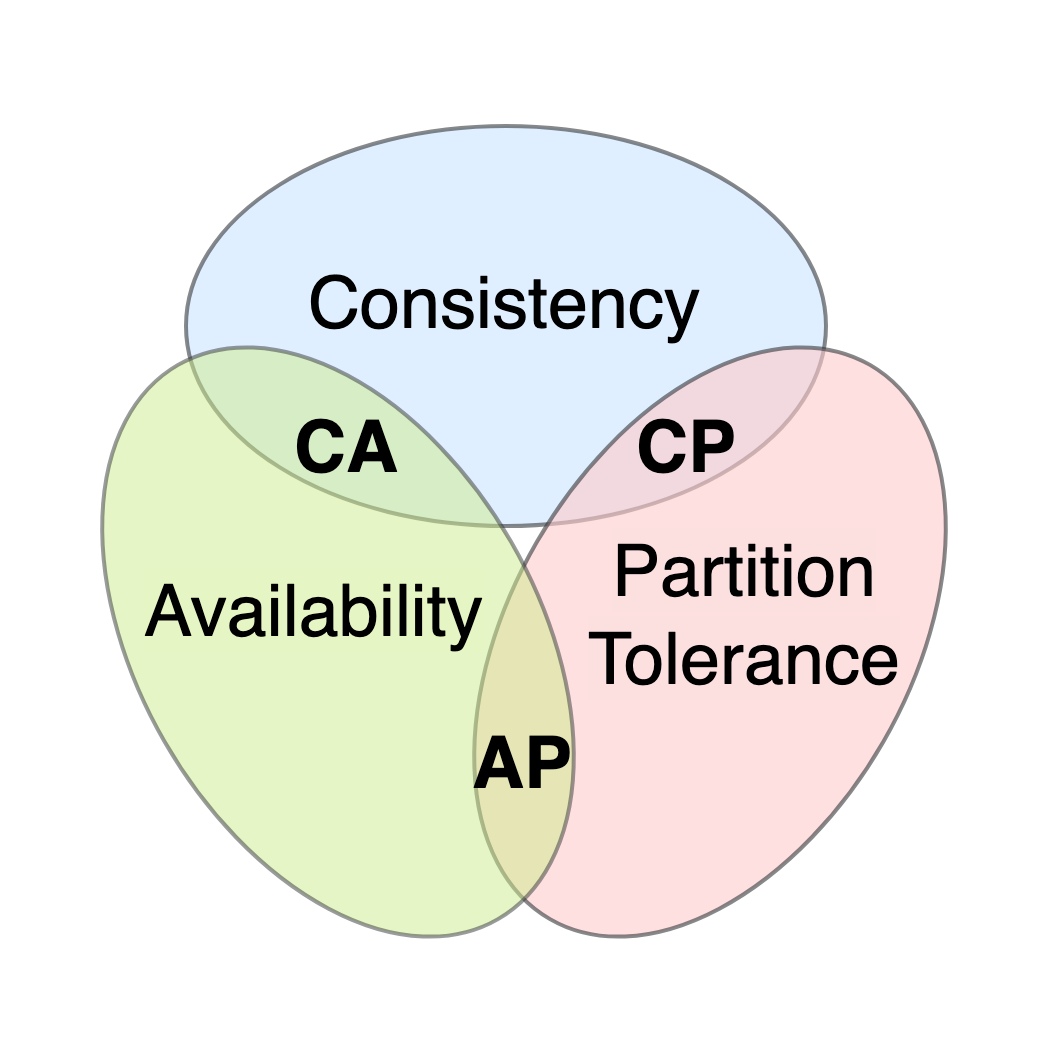
\includegraphics[width=0.4\linewidth]{assets/CAP_Theorem_Venn_Diagram}
	\caption{CAP theorem Venn diagram}
	\label{fig:captheoremvenndiagram}
\end{figure}
\chapter{Use cases}

\chapter{Databases design}

%TODO INCLUDE PDF WHEN COMPILING
%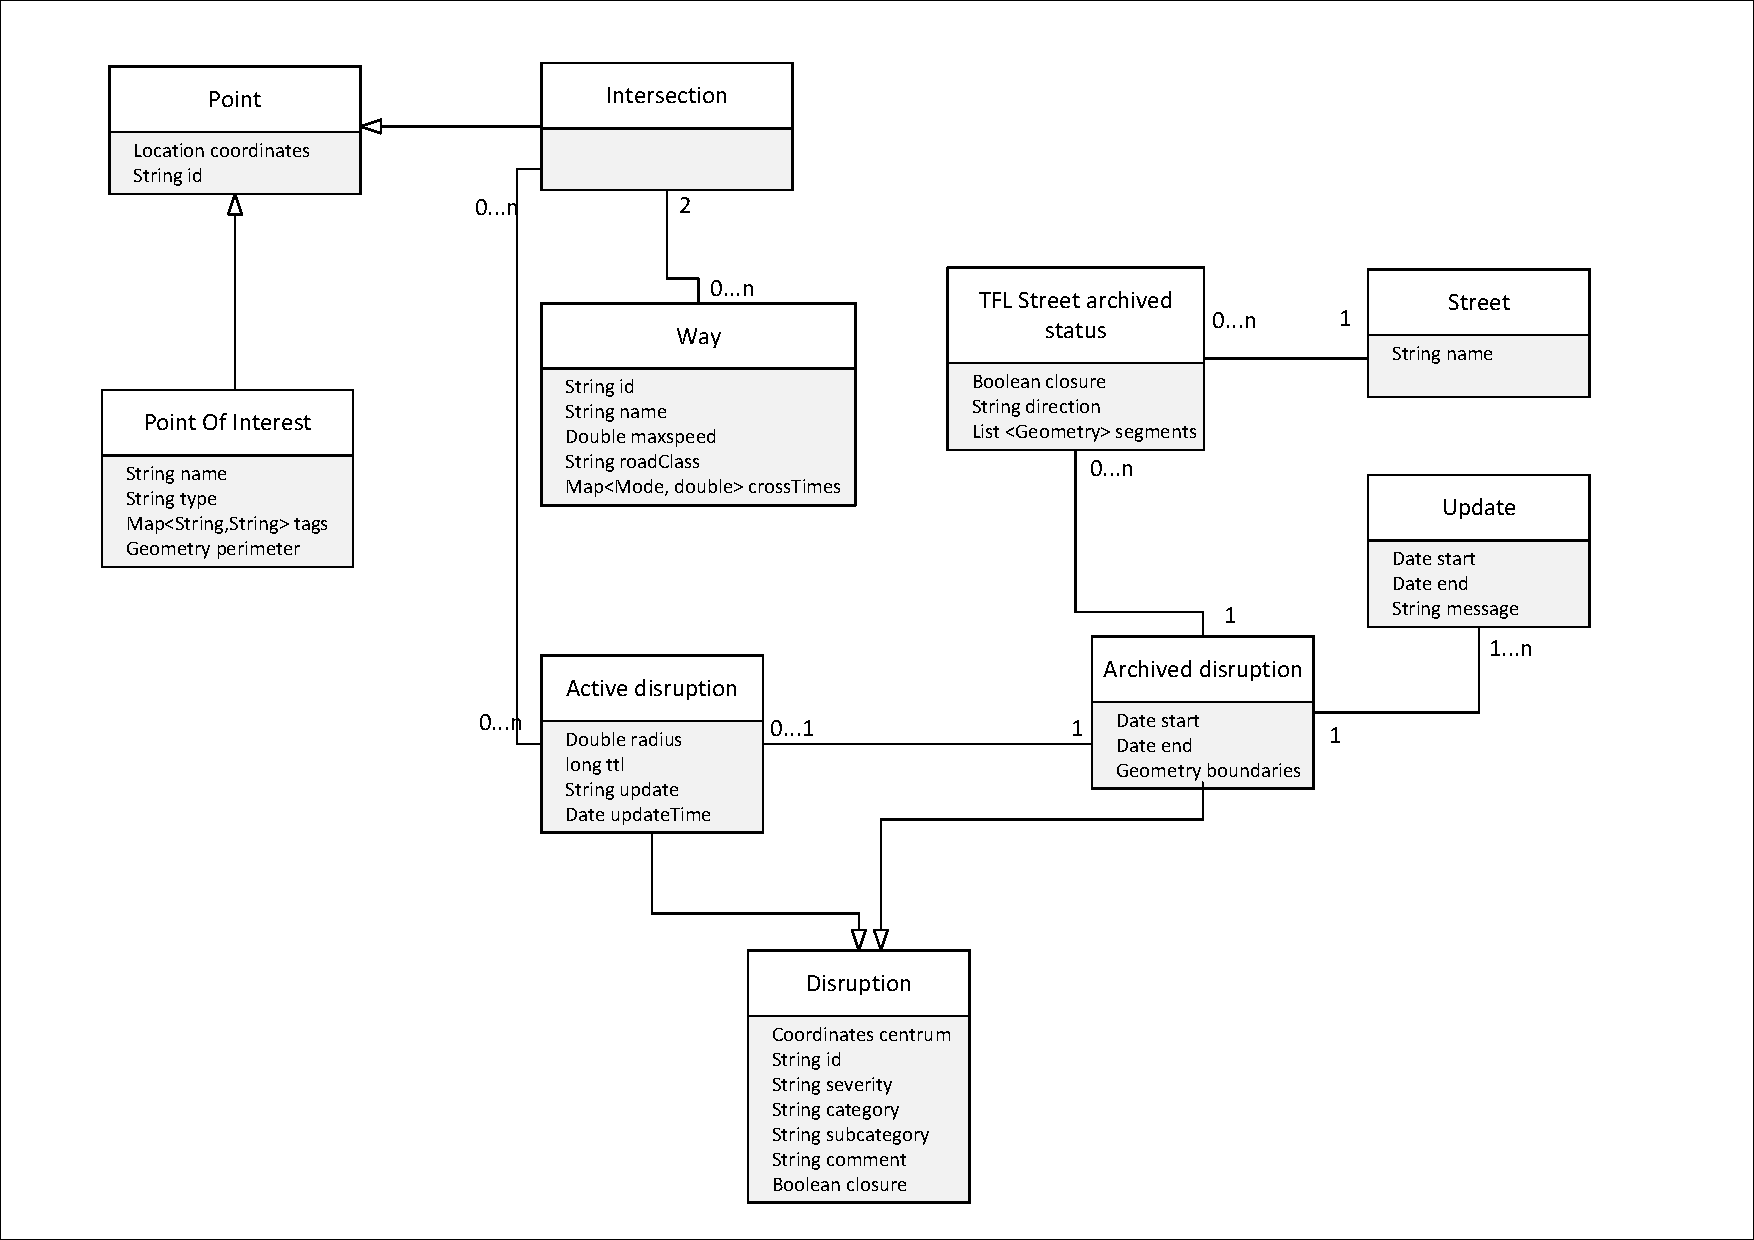
\includepdf[landscape=true,pagecommand=\thispagestyle{plain}]{assets/uml.pdf}

\chapter{Data model}

\paragraph{}
The data model section includes a description of the document collections, 
graph nodes and keys that are stored in the database. Two types of DBMSes have 
been selected for this purpose. 

\paragraph{Document DB}
MongoDB has been chosen as the database management system for the document 
database part, which stores information about the Point Of Interest and the 
concluded disruptions.

The decision to use a document database was based on its flexibility and 
ability to perform complex queries and works as a way to store an history of 
these informations.

\paragraph{Graph DB}
To manage the routing, where users can insert two points and the application will compute a travel route between them, a graph database managed using Neo4j has been selected to better support these features.

\section{Document database}

\paragraph{DBMS} Our choice for the \textit{database management system} to 
handle the document database was \textit{MongoDB}, since it is the most popular 
\textit{DBMS} of its kind and it also provides several functionalities useful 
for our use case, such as indexes and a powerful query engine.

\paragraph{Collections} In MongoDB we created the following collections:

\begin{itemize}
	\item POIs
	\item Disruptions
\end{itemize}

\subsubsection{Point of Interest}
The POIs collection looks like this:

\lstinputlisting{../../schema/example.poi.json}

Where the map \textit{tags} has not a particular structure, but it stores the 
\textit{OpenStreetMap}'s tag for that particular POI. It might store 
information such as its website, its opening hours, its physical dimensions, if 
it is accessible in a wheelchair etc...

\paragraph{Main fields}
\begin{itemize}
	\item \texttt{coordinates} a \textit{GeoJson} document of type 
	\texttt{Point} representing the geographical location of the object
	
	\item \texttt{name} the name of the object, if any
\end{itemize}

\subsubsection{Disruption}
The disruption collection is organized in the following structure:

\lstinputlisting{../../schema/example.disruption.json}

This representation might allow in the future to store additional optional 
values for certain kinds of POIs if the need arises, without any compatibility 
issue for the existing code; for example one might want to store a restaurant’s 
opening hours or the accessibility level for wheelchair users in a certain 
building.

\paragraph{Main fields}
\begin{itemize}
	\item \texttt{boundaries} a \textit{GeoJson} document that could be both of 
	class \texttt{Polygon} or \texttt{Multipolygon}, it represents the effected 
	area. It might not be present in all documents.
	
	\item \texttt{coordinates} the main point effected by the disruption, that 
	is where the application is supposed to draw the sign.
	
	\item \texttt{streets} a list of streets effected by the disruptions and if 
	are closed or not to the traffic
	
	\item \texttt{updates} an archive of updates that \textit{Transport for 
	London} has published
\end{itemize}

\section{Graph database}

\paragraph{DBMS} Our choice for the \textit{database management system} to 
handle the graph database was \textit{Neo4j}, since it can easly handle a huge amount of nodes.


\paragraph{Data} The graph DB is mainly used to store the road network of London and the current active disruption, this is needed so that the routing algorithm can avoid adding to the frontier nodes in an area affected by a closure or increase the weight of nodes in areas affected by critical disruptions.

\paragraph{Schema}For the map side of things we store one class of node and one class of relationship:

\begin{itemize}
	\item \textbf{Intersection }(due to a mistake it is actually called Point 
	in the database) represents the connection between one or more ways, it is 
	a \textit{vertex} of the graph
	
	\lstinputlisting{../../schema/example.point}
	
	\begin{itemize}
		\item \texttt{coord} Those are the geographical coordinates of the 
		node
	\end{itemize}
	
	\item \textbf{Connects} represents the connection between two Insersection. 
	It stores informations like its name and the cost of traversing it and 
	eventual access restrictions, like one way streets or motor-only roads
	
	\lstinputlisting{../../schema/example.connects}
	
	\begin{itemize}
		\item \texttt{maxspeed} It is the maximum speed on that stretch of road 
		expressed in meters per second
		
		\item \texttt{crossTime} It is the estimated crossing time of the edge 
		for each transportation mode. If the cross time is $\infty
		$ then it means 
		that the road has an access restriction in that direction, such has no 
		entry signs.
		
		It was used to use with the \textit{GDS}' implementation of 
		\textit{A*}, since we have implemented our version of \textit{A*} we 
		only check for $\infty$
		
		\item \texttt{class} The road class in the hierarchy where 
		\textit{motorway} is at the top.
	\end{itemize}
	
\end{itemize}

For the disruption handling we have the following nodes and relationships:

\begin{itemize}
	\item \textbf{Disruption} a node in the graph containing all the 
	informations about an active disruption
	
	\lstinputlisting{../../schema/example.disruption}
	
	We save in this edge all the information that could be of immediate help to 
	the user, to avoid making another query to the other databases when 
	requesting a preview of the data. In particular we store:
	
	\begin{itemize}
		\item \texttt{ttl} It is the \textit{Time to live}, that is the number 
		of seconds that remains to programmed end of the disruption, so that if 
		there are problems in the \textit{driver TIMS} the \textit{DBMS} can 
		drop it
	\end{itemize}
	
	\item \textbf{isDisrupted} is a relation between a Point and a Disruption, 
	telling that the road is being affected by a disruption.
	
	We don't store any information on those edges.

\end{itemize}
	
\begin{figure}[H]
	\centering
	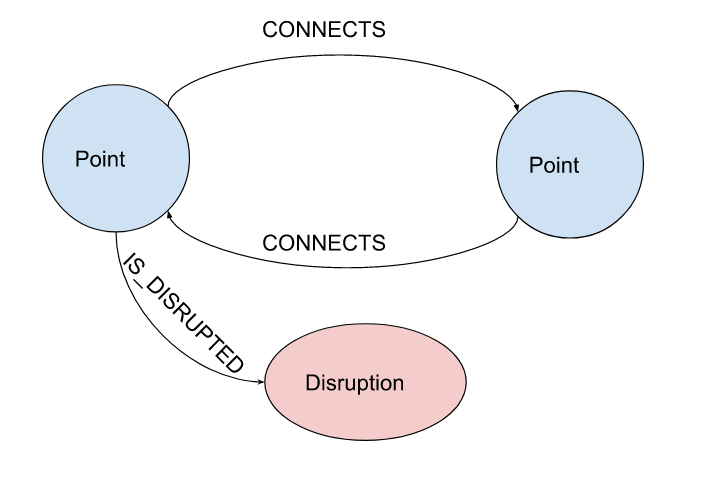
\includegraphics[width=0.7\linewidth]{assets/schemaneo4j}
	\caption{A possible portion of graph}
	\label{fig:schemaneo4j}
\end{figure}






\chapter{Distributed database}
\chapter{Overall platform architecture}

The application has been developed utilizing the Java programming language and the Intellij integrated development environment. As outlined in the Data Model section, MongoDB and Neo4j were chosen as the NoSQL database management systems for data storage and management. It was previously stated that there are three replicas implemented for MongoDB, and a single replica for Neo4j.
\chapter{Framework used}
\part{Implementation}

\chapter{Queries on graph database}

In this chapter are presented the relevant queries for the
Neo4j graph database.

\section{Routing}

Our routing query is used to compute a suboptimal path between two points on the map, given as input to the query, using the algorithm known as \textbf{Anytime A*}.

\begin{figure}[H]
	\lstinputlisting{../../queries/routing.cypher}
	\caption{Cypher query}
\end{figure} 

The procedure \textit{lodonSafeTravel.route.anytime} has been implemented as show below:

%\begin{figure}[H]
\lstinputlisting[linerange={50,163}, language=Java]
	{../../routingNeo4jProcedure/src/main/java/londonSafeTravel/RoutingAStart.java}
%	\caption{implementation of the procedure}
%\end{figure} 

\section{Point finding}

\paragraph{}
To ensure that the user selects a reachable point in the network given the user's transportation mode, we use \textit{connects} relationships between points in the graph to reduce the probability of selecting an unreachable point.

\begin{figure}[H]
	\lstinputlisting{../../queries/nearest_point.cypher}
	\caption{Cypher query}
\end{figure} 

\paragraph{}
For example, we in the user selects a pathway in a park and \textit{motor vehicle} is selected as transportation mode, the query will return the node relative to the nearest road open to motor traffic.

\paragraph{}
As stated in the previous chapters, a restriction of access for a certain mode of transportation is represented in the graph as cross time of positive infinity.

\paragraph{}
The function \textit{nearestNode} in Java has been implemented as show below:
%\begin{figure}[H]
\lstinputlisting[linerange={114-147}, language=Java]
{../../src/libCommon/src/main/java/londonSafeTravel/dbms/graph/ManageRouting.java}
%	\caption{implementation of the procedure}
%\end{figure} 

\chapter{Queries on Document database}
In this chapter are presented the relevant queries for the
MongoDB document database.

\section{POIs in a certain area}
\textit{Visualize the information of POIs in a given area}

%\begin{figure}[H]
\lstinputlisting[linerange={84-102}, language=Java]
{../../src/libCommon/src/main/java/londonSafeTravel/dbms/document/PointOfInterestDAO.java}
%	\caption{implementation of the procedure}
%\end{figure} 

\paragraph{}
The same query wrote in Mongo Query Language:
\begin{figure}[H]
\begin{lstlisting}
	db.PointOfInterest.find(
	{
		"coordinates": {
			$geoWithin: {
				$polygon: [
				[minLong, minLat],
				[maxLong, minLat],
				[maxLong, maxLat],
				[minLong, maxLat],
				[minLong, minLat]
				]
			}
		}
	}
	)
\end{lstlisting}
\caption{POIs' MongoDB query}
\end{figure}

\section{The heatmap}
\textit{Build a heatmap of a certain class of disruption.}

%\begin{figure}[H]
\lstinputlisting[linerange={120-161}, language=Java]
{../../src/libCommon/src/main/java/londonSafeTravel/dbms/document/DisruptionDAO.java}
%	\caption{implementation of the procedure}
%\end{figure} 

\paragraph{}
The same query wrote in Mongo Query Language:
\begin{figure}[H]
	\begin{lstlisting}
db.Disruption.aggregate([
{ $match: { category: classDisruption } },
{ 
	$project: {
		latB: { 
			$multiply: [ { 
				$floor: { 
					$divide: [ { 
						$arrayElemAt: 
						[ "$coordinates.coordinates", 1 ]
					 }, 
				 lenLat ] } },
			  lenLat ] },
		lngB: { 
			$multiply: [ { 
				$floor: { 
					$divide: [ { 
						$arrayElemAt: [ 
						"$coordinates.coordinates", 0 ] 
					}, lenLong ] } },
				 lenLong ] }
	}
},
{ 
	$group: {
		_id: { latB: "$latB", lngB: "$lngB" },
		count: { $sum: 1 }
	}
},
{
	$project: {
		count: 1,
		latitude: "$_id.latB",
		longitude: "$_id.lngB"
	}
}
])
\end{lstlisting}
\caption{Heatmap MongoDB query}
\end{figure}

\section{The most common disruptions}
\textit{Return a list witch contains the most common disruption in order to severity.}

%\begin{figure}[H]
\lstinputlisting[linerange={75-114}, language=Java]
{../../src/libCommon/src/main/java/londonSafeTravel/dbms/document/DisruptionDAO.java}
%	\caption{implementation of the procedure}
%\end{figure} 

\paragraph{}
The same query wrote in Mongo Query Language:
\begin{figure}[H]
	\begin{lstlisting}
		db.Disruption.aggregate([
		{
			$match: {
				coordinates: {
					$geoWithin: {
						$polygon: [
						[minLong, minLat],
						[maxLong, minLat],
						[maxLong, maxLat],
						[minLong, maxLat],
						[minLong, minLat]
						]
					}
				}
			}
		},
		{
			$group: {
				_id: { severity: "$severity", category: "$category" },
				count: { $sum: 1 }
			}
		},
		{
			$group: {
				_id: "$_id.severity",
				count: { $max: "$count" },
				type: { $first: "$_id.category" },
				severity: { $first: "$_id.severity" }
			}
		},
		{
			$sort: { count: -1 }
		},
		{
			$project: {
				_id: 0,
				severity: 1,
				type: 1,
				count: 1
			}
		}
		])
	\end{lstlisting}
	\caption{Common disruptions' MongoDB query}
\end{figure}

\section{Time series}
\textit{Returns, for each hour of the day, the average number of disruptions that were active at that time of day. Optionally the user can filter by disruption class to produce a graph relative only the specified class.}

%\begin{figure}[H]
\lstinputlisting[linerange={25-143}, language=Java]
{../../src/libCommon/src/main/java/londonSafeTravel/dbms/document/LineGraphDAO.java}
%	\caption{implementation of the procedure}
%\end{figure} 

\paragraph{}
The same query wrote in Mongo Query Language:
%\begin{figure}[H]
\lstinputlisting
{../../query.js}
%	\caption{Time series' MongoDB query}
%\end{figure}

\part{Conclusion}

\section{The Benefits of Using Graph and Document Databases in Transportation Systems}
In addition to meeting all objectives, the use of a graph database in our application has also brought several advantages. It has provided us with a highly flexible and scalable data storage solution, allowing us to easily add and modify data as needed. The graph structure of the database allows for efficient querying and indexing of data, enabling quick and accurate retrieval of information. This is particularly useful in the context of routing, as it allows for real-time updates to the routing information and the ability to quickly find alternative routes for users in the event of a disruption. We also used a document database to store the history of disruptions and Points of Interest (POIs).

By using a document database, we were able to store detailed information about each disruption and POI, including timestamps, location data, and any other relevant details. This allows us to maintain a historical record of disruptions and POIs, and provides us with valuable data for analyzing past disruptions and identifying patterns.

Furthermore, the use of a graph database also enables more advanced analytics and data visualization. The ability to create relationships between different data points and analyze them as a network provides a deeper understanding of the data and allows for more accurate predictions and recommendations. This can be particularly beneficial for the statistician, as it would enable them to make more informed decisions and proposals for improving traffic in London.

The use of both a graph database and a document database in our application allowed us to efficiently store and manage a wide variety of data, providing us with a comprehensive view of the transportation system and enabling more accurate predictions and recommendations for improving traffic in London.

\section{Possible expansions in the future}

In conclusion, the use of a graph and document database in our application has not only allowed us to meet our objectives but also brought several advantages such as efficient querying, advanced analytics, and scalability. It has opened up the possibility for more advanced functionalities to be implemented in the future, such as incorporating data on public transportation and the disruptions that it can cause, providing more comprehensive information and enabling more accurate predictions and recommendations for improving traffic in London.

\section{Possible query on public trasportations}

\textit{For each class of public transportation disruption, find the top 3  lines that are most affected.}


\begin{lstlisting}
db.Disruption.aggregate([
{
	$match: {
		typeDisruption: "PUBLIC_TRANSPORT"
	}
},
{
	$group: {
		_id: "$terminatedDisruption.category",
		count: { $sum: 1 },
		line: { $first: "$routes.line" }
	}
},
{
	$sort: { count: -1 }
},
{
	$limit: 3
}
])
\end{lstlisting}


\appendix
\part{Manual}

\chapter{User}

\begin{figure}[H]
	\centering
	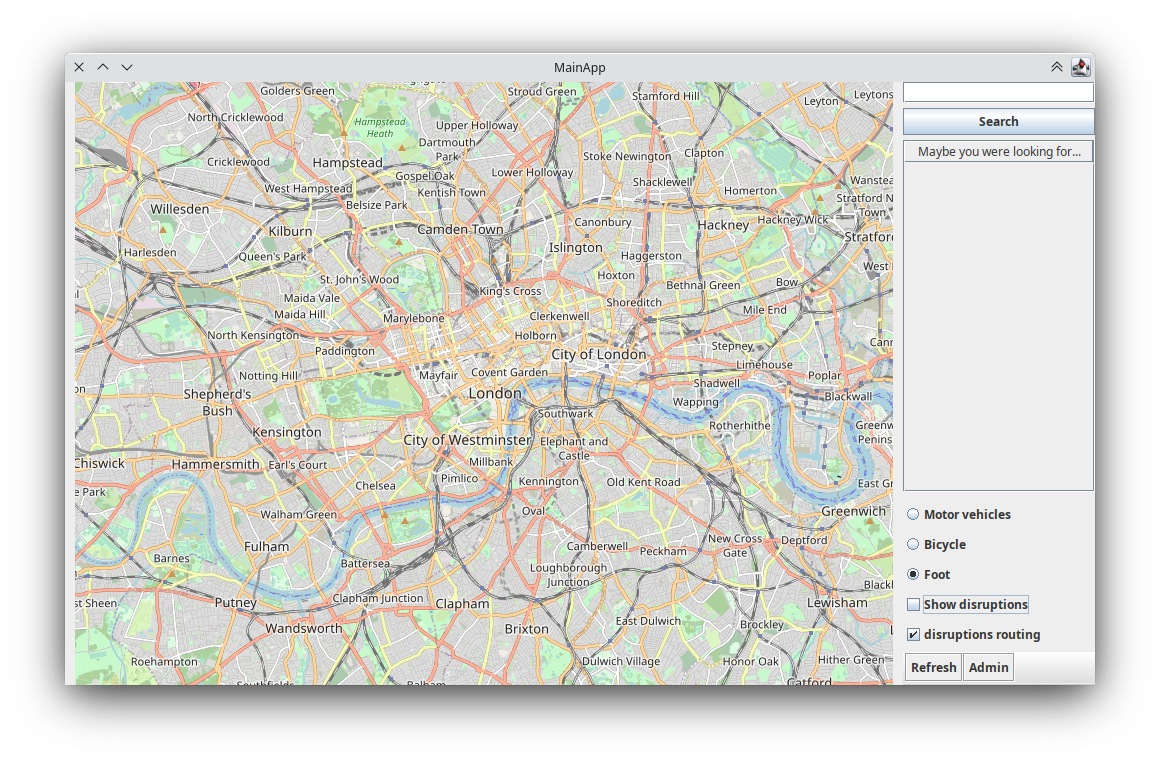
\includegraphics[width=\linewidth]{assets/mainapp0}
	\caption[]{Application just after launch}
	\label{fig:mainapp0}
\end{figure}

\paragraph{Introduction}
When launched the application automatically connects to the remote server and 
shows a map centered in London. The user can navigate the map with the typical 
\textit{drag 'n drop} that is common with those kind of applications and he can 
change the magnifying level with the scrolling wheel of the mouse.

\section{Point of interests}

\begin{figure}[H]
	\centering
	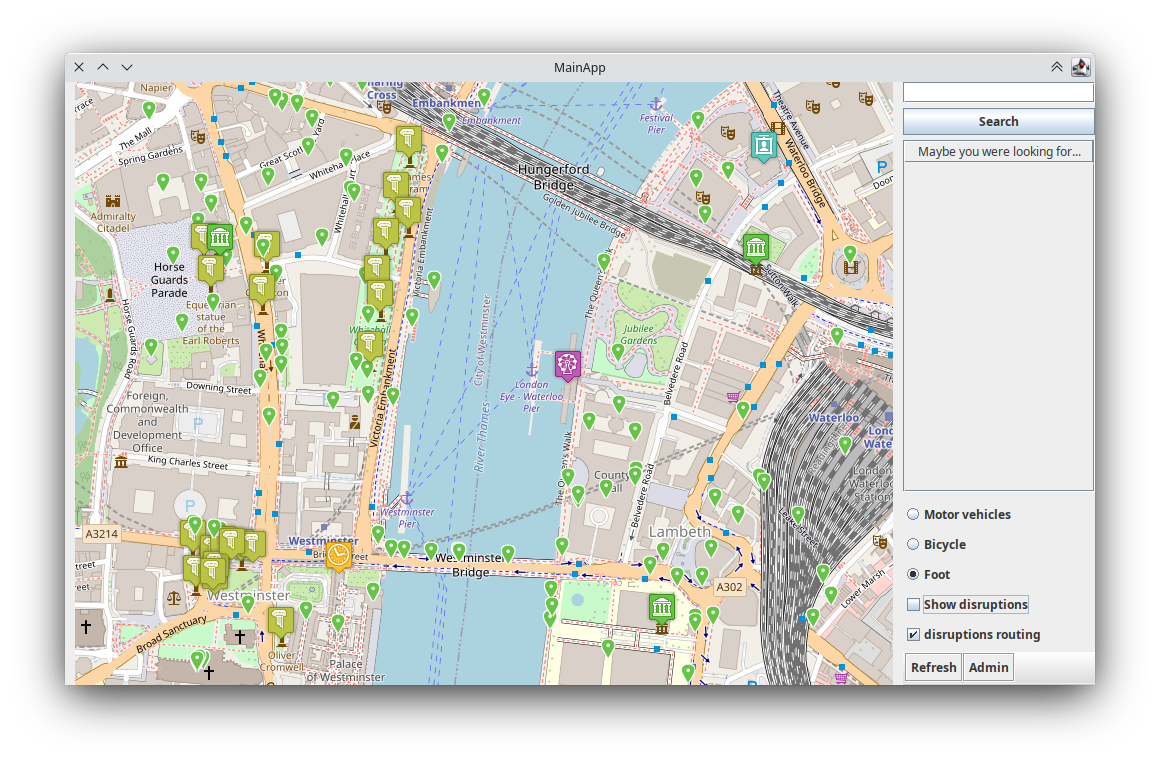
\includegraphics[width=\linewidth]{assets/mainapp1}
	\caption{Point of Interests near Westminster}
	\label{fig:mainapp1}
\end{figure}

\paragraph{Appearance}
The \textit{Point of Interest}s are being shown on the map only when an 
appropriate level of zoom is reached to avoid cluttering the map.

\paragraph{Information}
The user can access more information about a certain \textit{Point of Interest} 
by left-clicking on it. The application will then open an additional dialog 
with relevant information as seen in \ref{fig:mainappdialog1}

\begin{figure}[H]
	\centering
	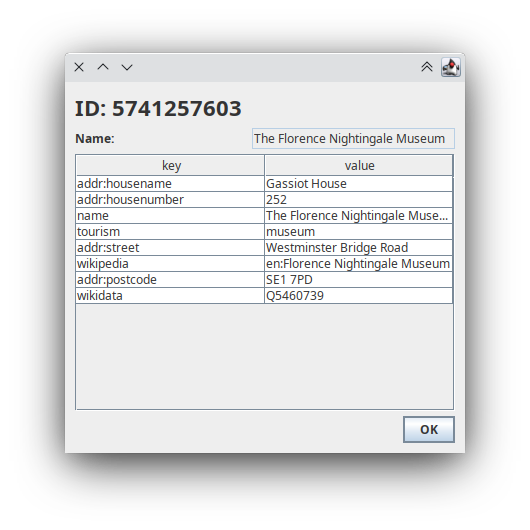
\includegraphics[width=0.5\linewidth]{assets/mainapp_dialog1}
	\caption[]{
		Informations regarding the "The Florence Nightingale Museum"
	}
	\label{fig:mainappdialog1}
\end{figure}

\section{Disruptions}

\paragraph{Appearance}
The user can make the currently active disruptions appear on the map by ticking 
the option called \textit{Show disruptions} located in the right panel. If 
needed the user can also force an update request by clicking on the button 
\textit{Refresh}.

The disruptions are color-coded according to their severity:

\begin{enumerate}
	\item \textbf{Grey} for disruptions with severity \textit{minimal}
	\item \textbf{Field drab} for disruptions with severity \textit{moderate}
	\item \textbf{Orange} for disruptions with severity \textit{serious}
	\item \textbf{Red} for disruptions with severity \textit{severe}
\end{enumerate}

\begin{figure}[H]
	\centering
	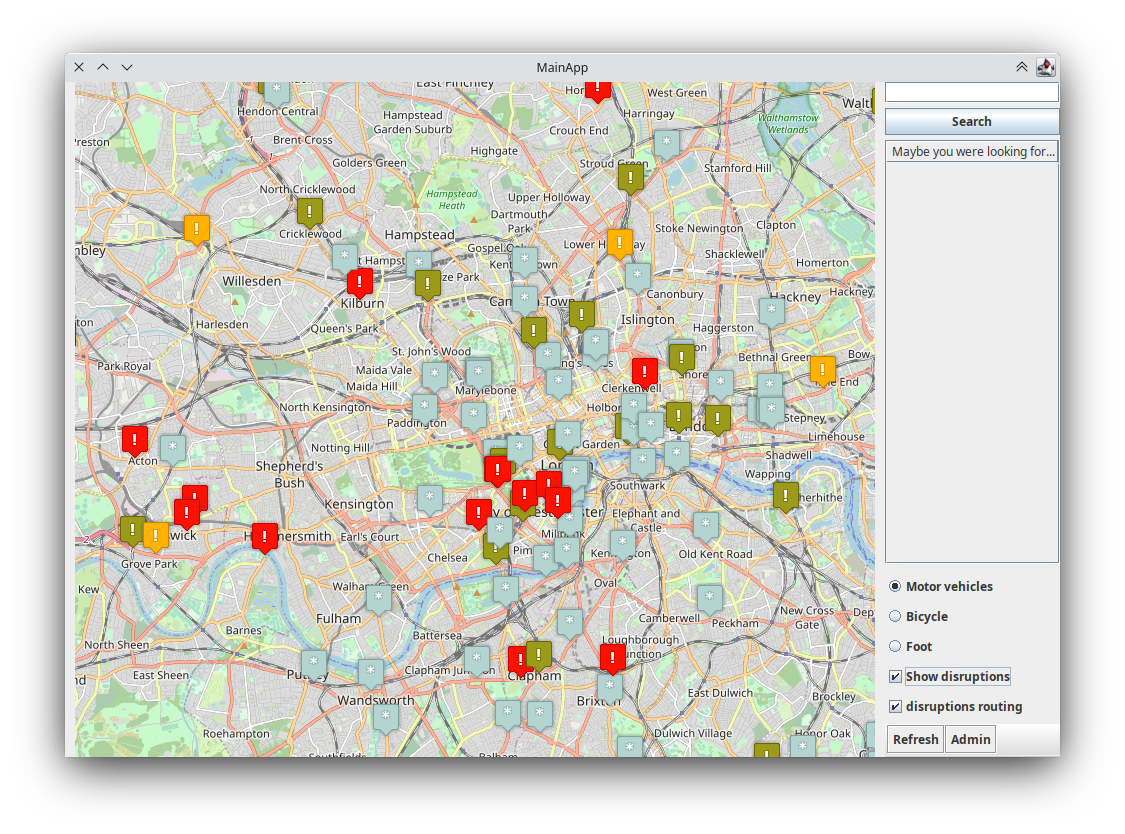
\includegraphics[width=\linewidth]{assets/mainapp2}
	\caption{Active disruptions in the afternoon of Janury 19th}
	\label{fig:mainapp2}
\end{figure}

\paragraph{Information}
The user can access more information about a certain \textit{disruption} 
by left-clicking on it. The application will then open an additional dialog 
with relevant information as seen in \ref{fig:mainappdialog2}

\begin{figure}[H]
	\centering
	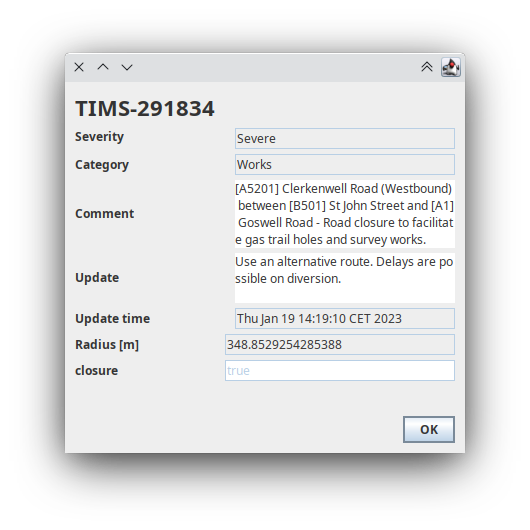
\includegraphics[width=0.5\linewidth]{assets/mainapp_dialog2.png}
	\caption[]{
		Information regarding disruption \textit{TIMS-291834}
	}
	\label{fig:mainappdialog2}
\end{figure}

\section{Routing}

\paragraph{Disruptions}
To make the routing consider delays caused by disruptions, tick the option 
called \textit{disruption routing}.

\paragraph{Mode}
The routing algorithm support three modes of transport: on foot, by bicycle or 
by car; select the appropriate option from the right panel.

\paragraph{Destination}
To route between two points, right-click on the departure point on the map then 
right click on the destination point on the map; then the routing will begin 
and the result will be rendered on the map as soon as it is available.

\begin{figure}[H]
	\centering
	\begin{subfigure}[b]{0.3\textwidth}
		\centering
		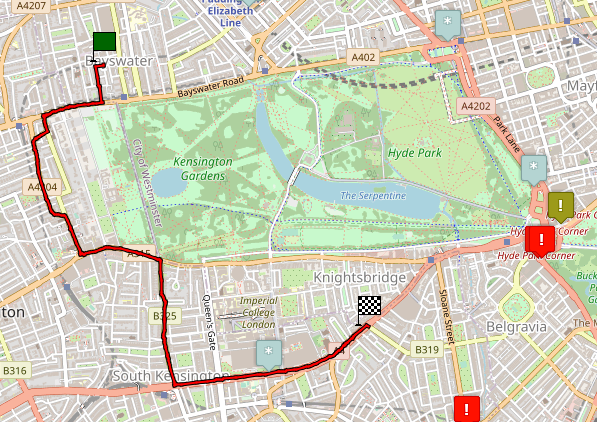
\includegraphics[width=\textwidth]{assets/routing_car.png}
		\caption{by car}
	\end{subfigure}
	\hfill
	\begin{subfigure}[b]{0.3\textwidth}
		\centering
		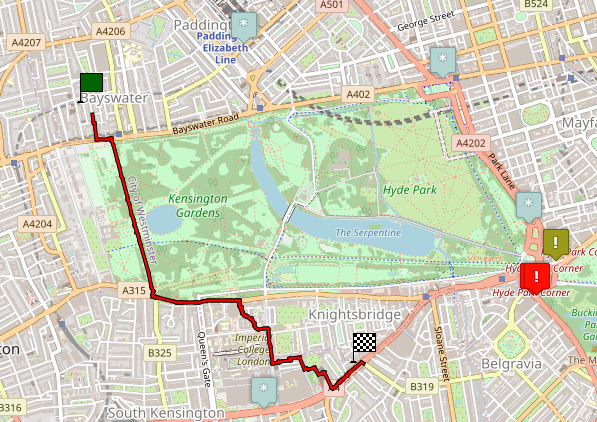
\includegraphics[width=\textwidth]{assets/routing_bike.png}
		\caption{by bicycle}
	\end{subfigure}
	\hfill
	\begin{subfigure}[b]{0.3\textwidth}
		\centering
		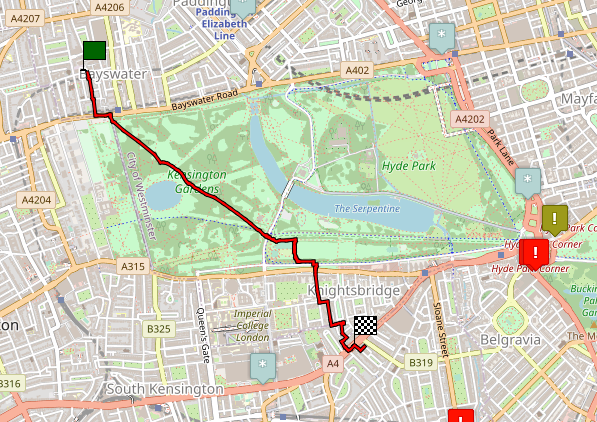
\includegraphics[width=\textwidth]{assets/routing_foot.png}
		\caption{on foot}
	\end{subfigure}
	\caption{Comparison between the three modes}
	\label{fig:routingsdiff}
\end{figure}

\paragraph{Results}
The path is rendered on the map as a red line, the estimated travel time is 
displayed in the right panel.

\begin{figure}[H]
	\centering
	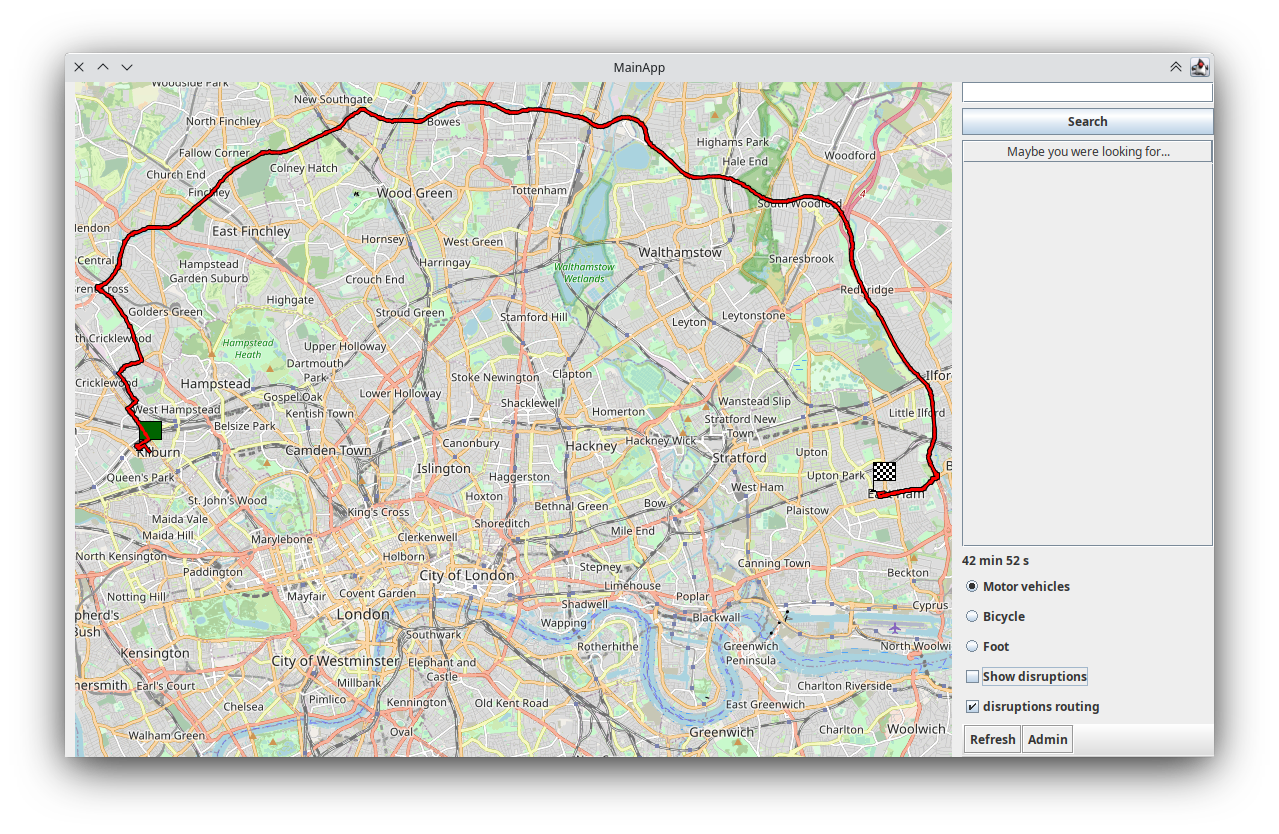
\includegraphics[width=\linewidth]{assets/mainapp3.png}
	\caption[]{
		Routing between Kilburn and East Ham.
		We can see how the routing procedure prefers faster motor-only roads 
		when traveling by car
	}
	\label{fig:mainappdialog3}
\end{figure}

\paragraph{Time estimation}
The travel time estimations considers several factors such as

\begin{itemize}
	\item The maximum speed for the given mode
	\item If in a vehicle, the speed limit
	\item If in a motor vehicle, the road class
	\item If enabled, the disruptions' severity
\end{itemize}

\begin{figure}[H]
	\centering
	\begin{subfigure}[b]{0.48\textwidth}
		\centering
		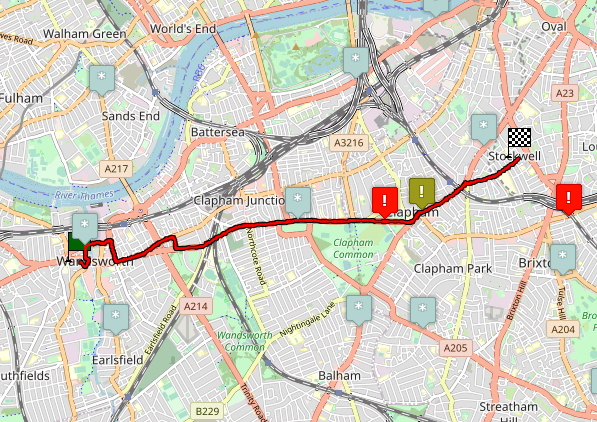
\includegraphics[width=\textwidth]{assets/routing_without_disruptions.png}
		\caption{disruptions off}
	\end{subfigure}
	\hfill
	\begin{subfigure}[b]{0.48\textwidth}
		\centering
		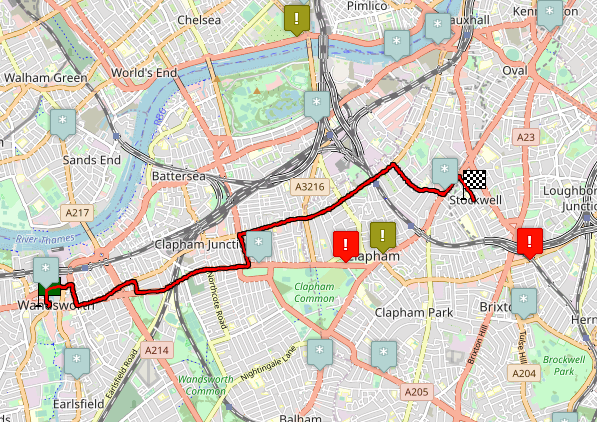
\includegraphics[width=\textwidth]{assets/routing_with_disruptions.png}
		\caption{disruptions on}
	\end{subfigure}
	\caption[]{Routing and disruptions}
\end{figure}

\pagebreak

\section{Search}

\paragraph{}
It is possible to search on the map for \textit{Point of Interest} by keyword.

\paragraph{Search}
To perform a search the user has to input his query in the\textit{Search} input 
box in the right panel and then click on the \textit{Search} button.

\paragraph{Result}
The map is centered on the most relevant \textit{Point of Interest}, other 
results are shown in a list in the right panel, below the search button.

\begin{figure}[H]
	\centering
	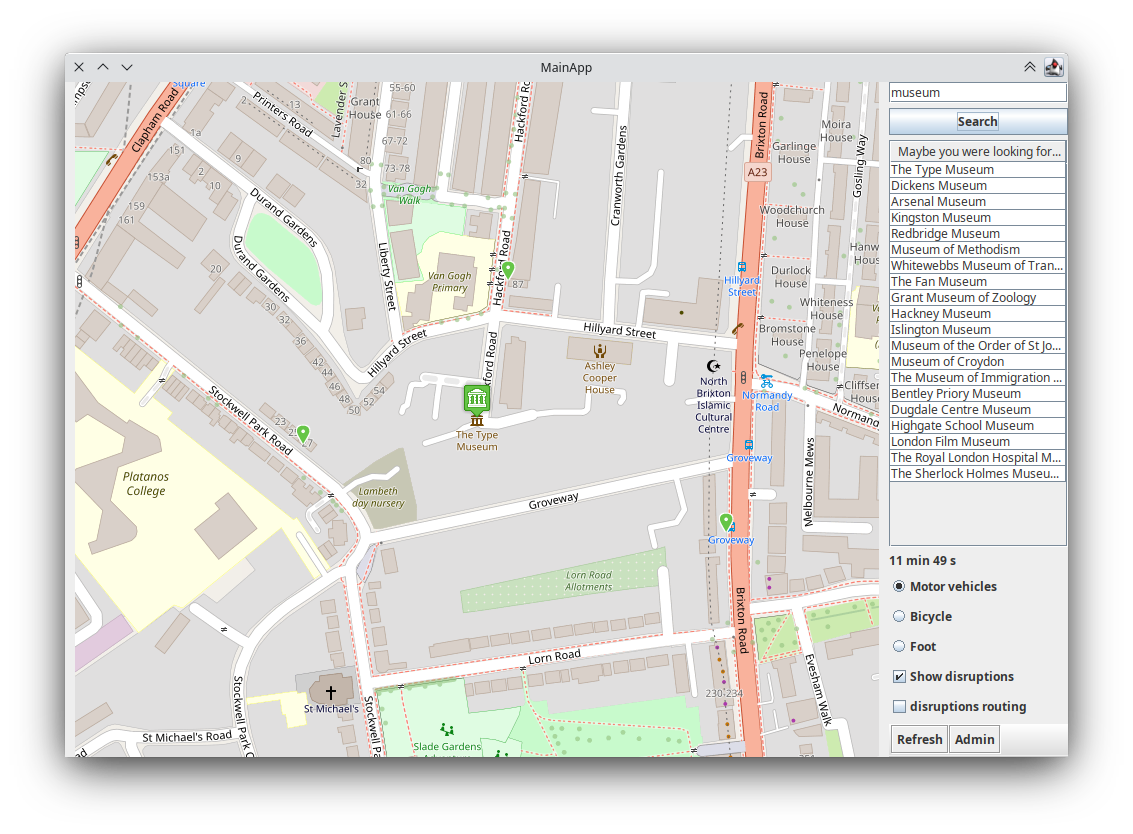
\includegraphics[width=\linewidth]{assets/mainapp4.png}
	\caption[]{
		Query results for \textit{Museum}
	}
	\label{fig:mainappdialog4}
\end{figure}

\chapter{Statistician}

\begin{figure}[H]
	\centering
	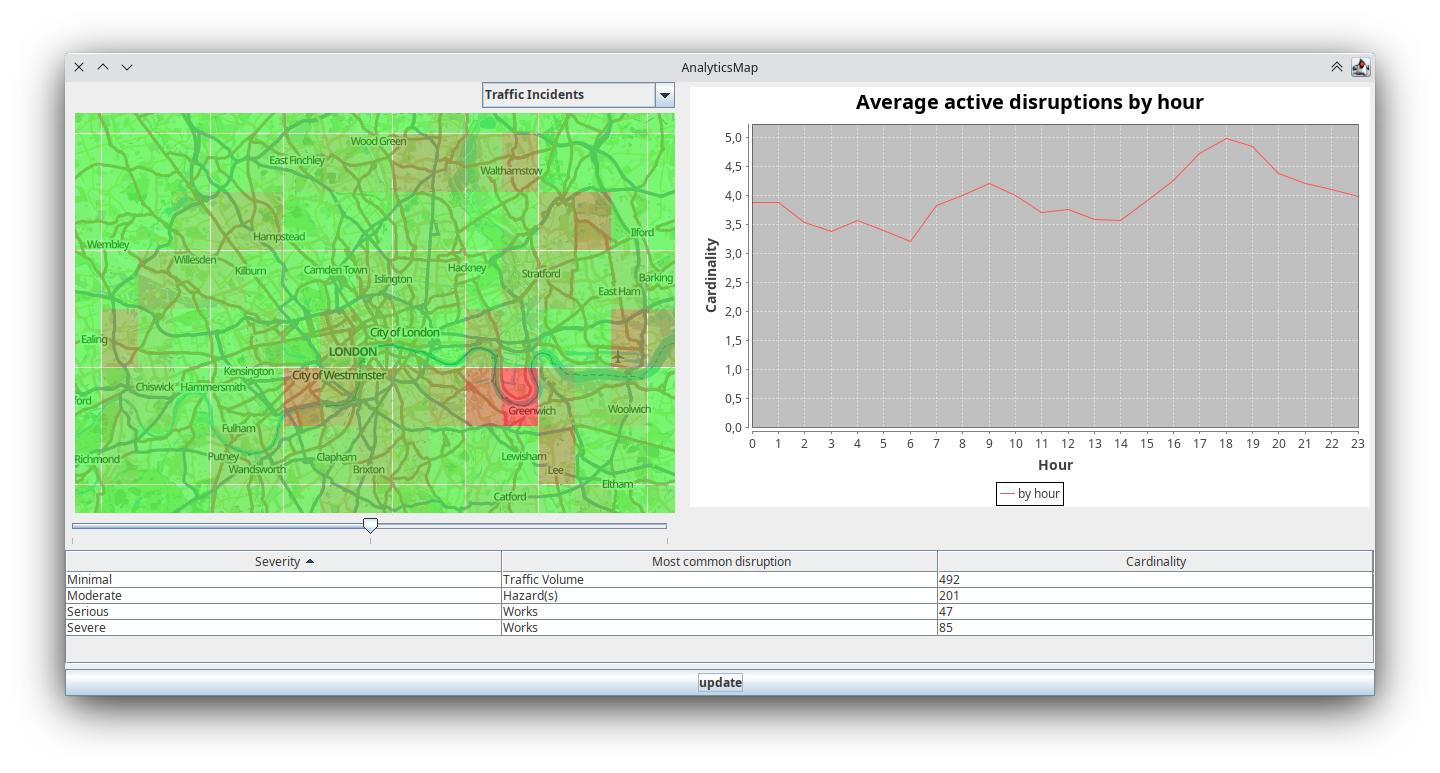
\includegraphics[width=\linewidth]{assets/anayitics0.png}
	\caption[]{}
	\label{fig:anal0}
\end{figure}

\paragraph{Access}
The authorized personnel can access the administrative window by clicking on 
the \textit{Admin} button and entering his credentials in the dialog. In the 
demo application is it possible to log-in with the following details:

\begin{lstlisting}[numbers=none, frame=single]
Username: admin
Password: admin
\end{lstlisting}

\paragraph{Layout}
The analytic window is divided in three main panels, one for each analytic 
provided by the application.

\section{Heat-map}

\paragraph{}
The heat-map is located in the top-left pane of the window. It shows a heat-map 
relative to the selected disruption; the green color represents an area where a 
the class of disruption never happened, the red color represents an area where 
most of the disruptions happened.

\paragraph{Category}
To select the \textit{category of disruption} to analyze, select it from the 
drop-down list above the map.

\paragraph{Precision}
To applications provides three levels of precision when computing the heat-map, 
to change it move the slider below the map; to the left is more precise, that 
is to render smaller squares, and to the right is less precise.

\paragraph{Movements}
As for the user's map, it is possible to move around via \textit{drag 'n drop}.

\section{Disruptions' time series}

\paragraph{}
The time series is located on the top-right pane of the window. It shows how 
common was a disruption in a certain hour of the day.

\paragraph{Category}
The category is the same as the one selected for the heat-map.

\section{Common disruptions in an area}

\paragraph{}
The result of this analytic are presented in the table located in the bottom 
pane of the window. It shows, for each category, how many disruptions happened 
in the selected area, and what was the most common sub-category for each one.

\paragraph{Boundaries}
To select the boundaries move the map around and adjust its zoom, unlike the 
others, to update the result press the \textit{update button}.  

\end{document}          
